\section{Contexto Histórico}
\begin{frame}\frametitle{Thickness}
	\begin{figure}
		\centering
		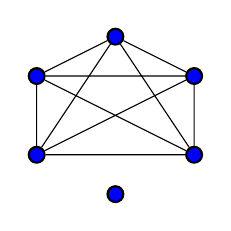
\begin{tikzpicture}
		\begin{scope}[every node/.style={circle,thick,draw,fill=blue,minimum size=2mm,inner sep=0pt}]
		\node(p1) at (0,0){};
		\node (p2) at (0,1){};
		\node (p3) at (1,1.5){};
		\node (p4) at (2,1) {};
		\node(p5) at (2,0) {};
		\node (p6) at (1,-0.5){};
		\end{scope}
		\draw \foreach \k [count=\j from 1] in {1,...,5}
		\foreach \kk in {\j,...,5}
		{(p\k)--(p\kk)};
		\end{tikzpicture}
		\quad\quad\quad
		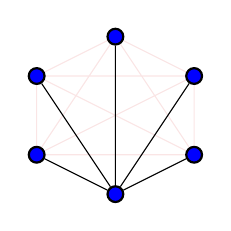
\begin{tikzpicture}
		\begin{scope}[every node/.style={circle,thick,draw,fill=blue,minimum size=2mm,inner sep=0pt}]
		\node(p1) at (0,0){};
		\node (p2) at (0,1){};
		\node (p3) at (1,1.5){};
		\node (p4) at (2,1) {};
		\node(p5) at (2,0) {};
		\node (p6) at (1,-0.5){};
		\end{scope}
		\draw[red!80!black,opacity=0.1] \foreach \k [count=\j from 1] in {1,...,5}
		\foreach \kk in {\j,...,5}
		{(p\k)--(p\kk)};
		\draw \foreach \kk in {1,...,6}
		{(p6)--(p\kk)};
		\end{tikzpicture}
	\end{figure}
	En 1961, Harary propone un problema:
	\begin{quotation}
		Demuestre la siguiente conjetura: Para cualquier gráfica $G$ con 9 vértices, $G$ o su gráfica complementaria $\overline{G}$\let\thefootnote\relax\footnote{$\overline{G}$:La gráfica inducida resultante de remover todas las aristas de $G$ de $K_n$} es no planar.
	\end{quotation}
	Harary, Battle y Kodoma y Tutte probaron, de manera independiente, que $K_9$ no es la unión de dos \emph{gráficas planares} (no es biplanar). En 1963, Tutte definió el \emph{thickness} de una gráfica, generalizando el término de biplanaridad. 
	\let\thefootnote\svthefootnote
\end{frame}
\begin{frame}\frametitle{Thickness Geométrico}
	En el año 2000, Dillencourt, Eppstein y Hirschberg dan el valor exacto del \emph{thickness geométrico} para gráficas completas.
	
 	Ellos definen el thickness, $\theta(G)$, de una gráfica $G$ como el mínimo número de gráficas planares en una descomposición de $G$. Por otro lado, definen el thickness geométrico, $\overline{\theta}(G)$, de $G$ como el número mínimo de gráficas \emph{planas} que existen en una descomposición de $G$, para todos los \emph{dibujos geométricos} de $G$.
\end{frame}
\begin{frame}
	\begin{figure}
		\centering
		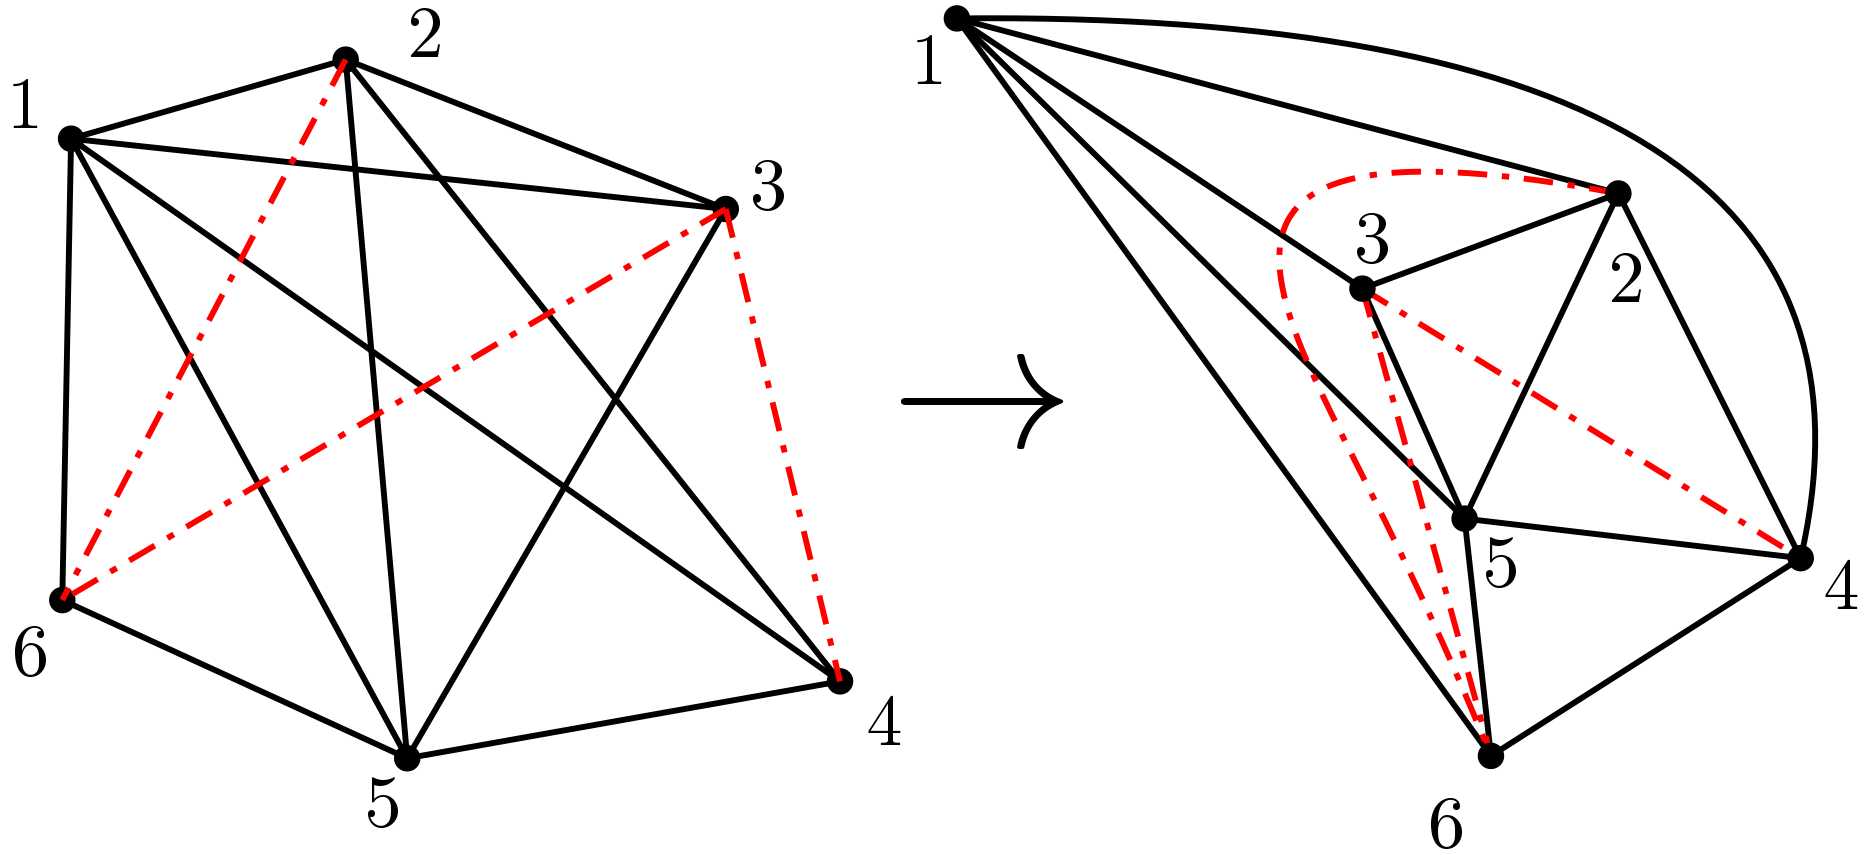
\includegraphics[width=0.6\textwidth]{images/K6_thicknes2}%
		~\vrule
		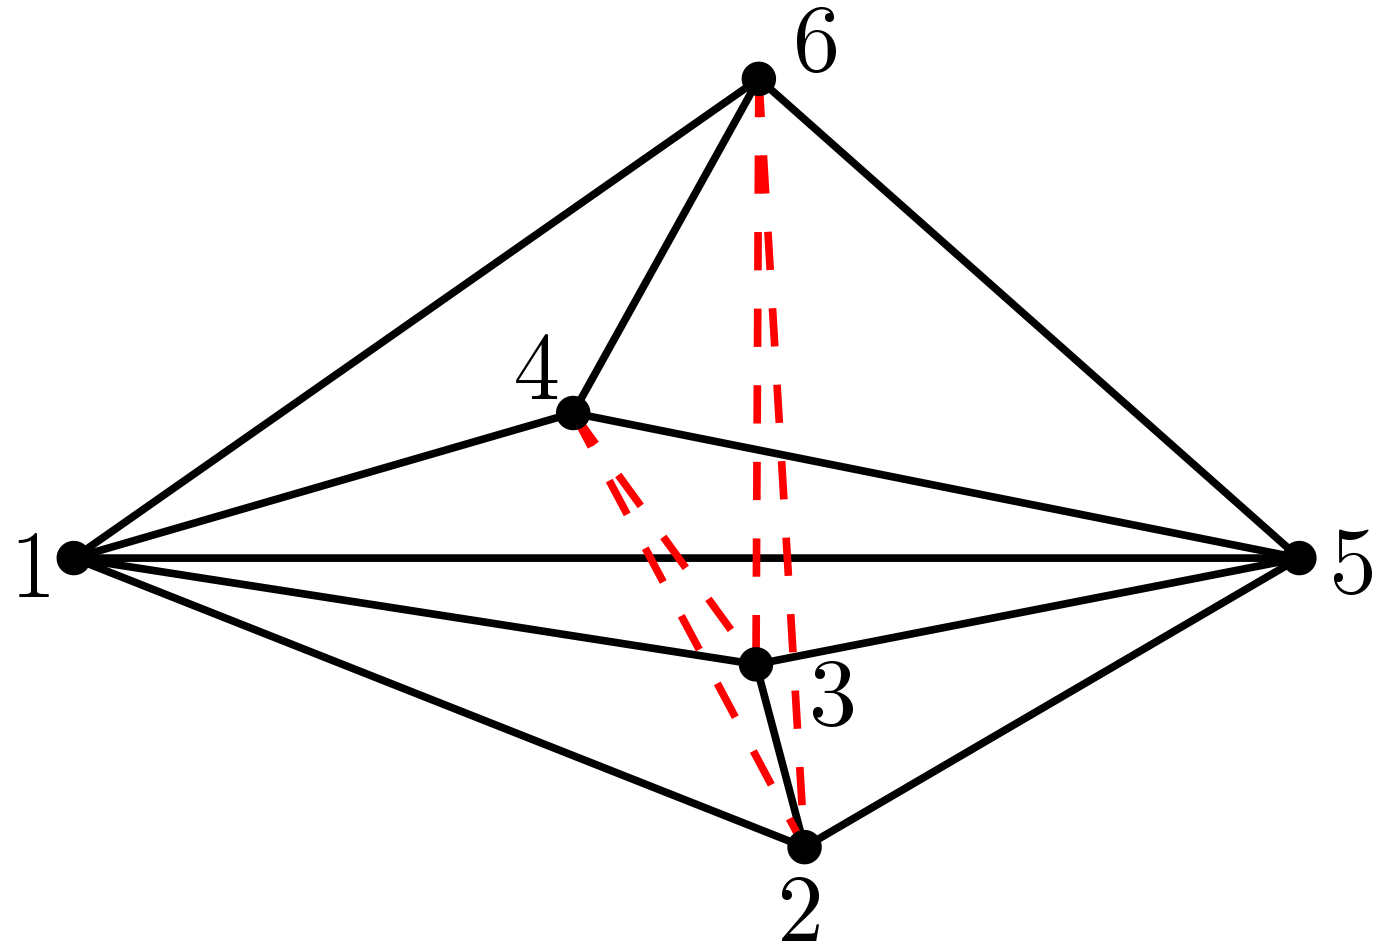
\includegraphics[width=0.4\textwidth]{images/K6_gthicknes2}
	\end{figure}
\end{frame}

\begin{frame}\frametitle{Gráfica de cruce}
Es posible abstraer la información de los cruces de gráficas geométricas usando un tipo de gráficas a las que llamamos \emph{gráficas de adyacencia}.

\begin{itemize}
	\item Las gráficas de adyacencia tienen como conjunto de vértices a las aristas de la gráfica completa que es inducida por algún conjunto $S$ de $n$ puntos.
\end{itemize}
Nosotros llamamos gráfica de cruce $E_{pp}(S)$ a la gráfica de adyacencia en la que existe una arista entre dos vértices cuando sus aristas correspondientes se cruzan.
\end{frame}

\begin{frame}
	\begin{figure}
	\centering
	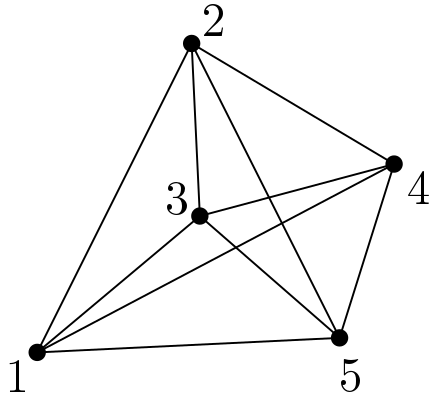
\includegraphics[width=0.2\textwidth]{images/K5}%
	~\vrule
	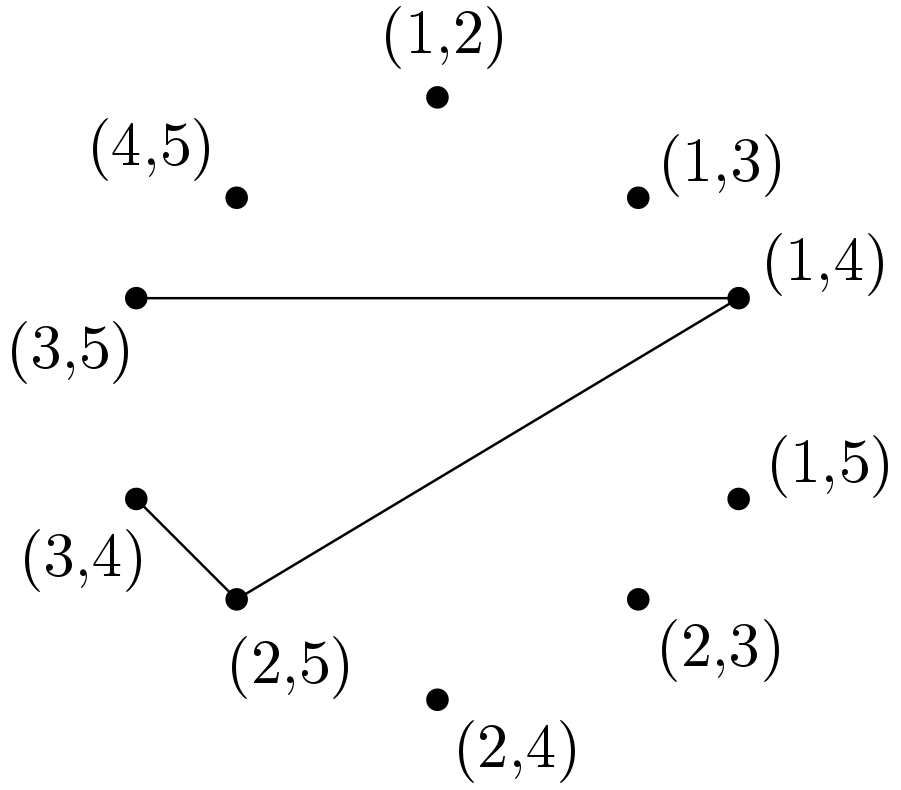
\includegraphics[width=0.3\textwidth]{images/EppK5}
	~\vrule
	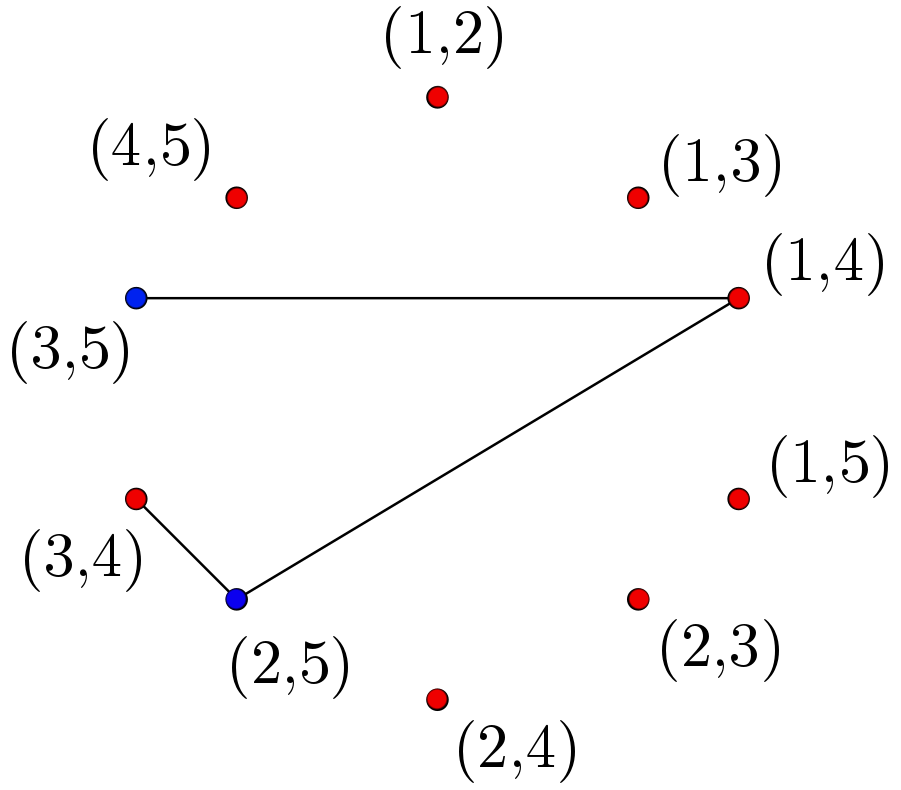
\includegraphics[width=0.3\textwidth]{images/EppK5_colored}
	\end{figure}
	Si encontramos una coloración propia de $E_{pp}(S)$ las clases cromáticas representan gráficas planas. Luego, el número cromático $\chi(E_{pp}(S))$\footnote{El número cromático, $\chi(G)$, de $G$ es el mínimo número de clases cromáticas en una coloración propia de $G$.} nos dice el mínimo número de gráficas planas que componen a la gráfica inducida por $S$.
	
	Finalmente: $\overline{\theta}(K_n(S)) = \min\{\chi(E_{pp}(S)) : S \text{ es un conjunto de $n$ puntos}\}$
\end{frame}

\begin{frame}{Gráficas de adyacencia}
\begin{figure}
	\centering
	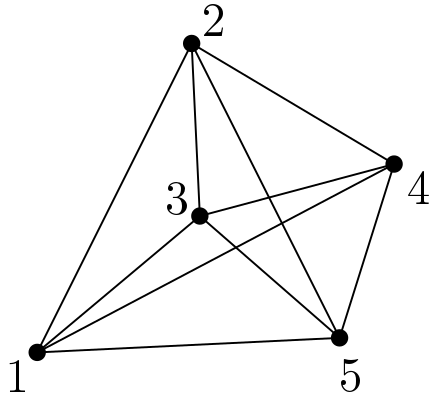
\includegraphics[width=0.2\textwidth]{images/K5}%
	~\vrule
	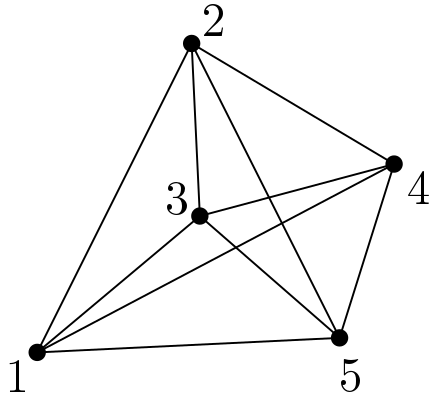
\includegraphics[width=0.2\textwidth]{images/K5}%
	~\vrule
	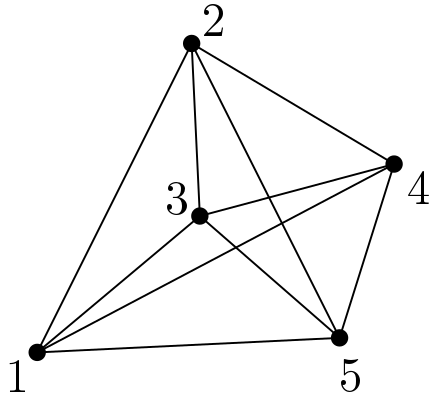
\includegraphics[width=0.2\textwidth]{images/K5}%
\end{figure}
Existen otras gráficas de adyacencia, si consideramos otro criterio para definir las aristas de la gráfica de adyacencia podemos obtener diferentes resultados.
\begin{itemize}
	\item $W(S)$: Existe una arista entre dos vértices si las aristas correspondientes comparten un vértice o son disjuntas. Las clases cromáticas son \emph{crossing families}.
	\item $I(S)$: Existe una arista entre dos vértices si las aristas correspondientes se intersectan. Las clases cromáticas son \emph{emparejamientos planos}.
	\item $D(S)$: Existe una arista entre dos vértices si las aristas correspondientes son disjuntas. Las clases cromáticas son \emph{thrackles}.
\end{itemize}


\end{frame}